\subsection{Adiabatic perturbations}\label{analytic_adia}
We now extend the above discussion to general $\gamma$, but in the
adiabatic limit ($t_c\to\infty$). We eliminate variables from 
Eq. \ref{lin_mass}---\ref{lin_energy} in favor of $\delta v_z$ 
and $\Delta \equiv \nabla\cdot\delta\bm{v}$ to obtain
\begin{align}
  &\Delta\left(1 + \frac{\gamma c_s^2 k_x^2}{D}\right) = \frac{d\delta
    v_z}{dz} + \frac{\ii k_x^2}{D}\left(\ii c_s^2 \frac{d\ln\rho}{dz}
    - \frac{r}{k_x}\frac{d\Omega^2}{dz}\right)\delta v_z,\label{adia_iso1}\\
  & -\frac{\sigma^2}{c_s^2}\delta v_z = \gamma \frac{d\Delta}{dz} +
  \frac{d}{dz}\left(\frac{d\ln\rho}{dz}\delta v_z\right) +
  \left(\gamma-1\right)\frac{d\ln\rho}{dz} \Delta.\label{adia_iso2}
\end{align}
%{\bf note: incompressible mode, set delta to zero. only works for
% constant gravity.}

We make the low-frequency approximation and the replacement 
$D\to \Omega_k^2$ in Eq. \ref{adia_iso1}---\ref{adia_iso2}. For
simplicity we do this before combining these equations later. We  
show in Appendix \ref{adia_improve} that making these approximations
after combining  Eq. \ref{adia_iso1}---\ref{adia_iso2} adds unecessary
complexity for thin disks. Here, we also use the fact that in the
global disk, 
\begin{align}
  r\frac{\p \Omega^2}{\p z} = -\frac{\p \ln\rho}{\p z} \frac{qc_s^2}{r},
\end{align}
for the power-law prescription of the midplane sound-speed for
$\Gamma=1$.  

Making the above substitutions and eliminating $\Delta$ between Eq. \ref{adia_iso1}---
Eq. \ref{adia_iso2} we obtain, in terms of dimensionless variables defined
previously, an equation for $\delta v_z$, 
\begin{align}
  0 =& \dd v_z^{\prime\prime} + \left(1 + \ii \epsilon q
    \hat{k}\right)\left(\ln\rho^{\prime}\delta v_z\right)^\prime\notag\\
  &+\left\{\hat{\sigma}^2\left(\frac{1}{\gamma}+\hat{k}^2\right)\right.\notag\\
  &\phantom{0=}\left.-\left(\frac{\gamma-1}{\gamma}\right)\left[\ln\rho^{\prime\prime}+\hat{k}^2\left(1-\frac{\ii\epsilon  
          q}{\hat{k}}\right)\ln\rho^{\prime 2}\right]\right\}\delta v_z.\label{adia_iso3}
\end{align}

We multiply Eq. \ref{adia_iso3} by $\rho\delta v_z^*$ and
integrate vertically, assume boundary terms vanish when integrating by
parts, to obtain
\begin{align}
  &\hat{\sigma}^2\left(\frac{1}{\gamma} +
    \hat{k}^2\right)\int_{\zhat_1}^{\zhat_2}\rho|\delta
  v_z|^2 d\zhat \notag\\
  &=  \left(\frac{\gamma-1}{\gamma}\right)
  \int_{\zhat_1}^{\zhat_2}\rho|\delta v_z^\prime|^2 d\zhat
  +\frac{1}{\gamma}\int_{\zhat_1}^{\zhat_2}\frac{1}{\rho}|(\rho\delta
  v_z)^\prime|^2 d\zhat\notag\\
  &\phantom{=} +
  \left(\frac{\gamma-1}{\gamma}\right)\hat{k}^2\left(1-\frac{\ii\epsilon
      q}{\hat{k}}\right) \int_{\zhat_1}^{\zhat_2}\rho\ln\rho^{\prime
    2}|\delta v_z|^2 d\zhat\notag\\
  &\phantom{=} + \ii\epsilon q \hat{k}
  \int_{\zhat_1}^{\zhat_2}\ln\rho^\prime(\rho\delta v_z^*)^\prime
  \delta v_z d\zhat.\label{adia_integral}
\end{align}
When $q\equiv0$, all the terms on the right-hand-side (RHS) are real. Then
$\hat{\sigma}^2$ is real, and  $\hat{\sigma}^2>0$ if $\gamma>1$. As
expected, a sub-adiabatically stratified disk is stable in the absense
of vertical shear. In the presence of vertical shear $q\neq0$ and
$\hat{\sigma}$ is generally complex, which implies the possibility of
instability.  

Note that when $\gamma>1$ and $q=0$, the term with $\ln\rho^{\prime
  2}$ in the integrand (third term on the RHS) represents
stabilization by the vertical entropy gradient (real bouyancy frequency). 
It gives an imaginary contribution to $\hat{\sigma}$ when $q\neq0$,
but this is a factor $|\epsilon/\hat{k}|$ smaller than the real
(stabilizing) contribution, 
since $\epsilon\ll 1$ for a thin disk and we (usually) consider
$\hat{k}\gg1$. Thus, instability is expected to be associated with the 
last term on the RHS of Eq. \ref{adia_integral}. 

\subsubsection{Explicit solutions in the thin-disk limit}
We can construct solutions in the thin-disk limit, in which 
$\ln(\rho/\rho_0) \simeq -\zhat^2/2$. Eq. \ref{adia_iso3} becomes   
\begin{align}
  0 = \delta v_z^{\prime\prime} - \zhat A \delta v_z^\prime + \left(B
    - C \zhat^2\right)\delta v_z,
\end{align}
with
\begin{align}
  &A \equiv 1 + \ii \epsilon q \hat{k},\\
  &B \equiv \hat{\sigma}^2\left(\frac{1}{\gamma} + \hat{k}^2\right) -
  \left(\frac{1}{\gamma} + \ii \hat{k} \epsilon q\right)\\
  &C \equiv \frac{\left(\gamma-1\right)}{\gamma}\hat{k}^2\left(1 - \frac{\ii
      \epsilon q}{\hat{k}}\right).\label{adia_thin}
\end{align}
Let
\begin{align}
  \delta v_z(\zhat) =
  g(\zhat)\exp\left(\frac{\alpha\zhat^2}{2}\right), \label{adia_ansatz}
\end{align}
where $\alpha$ is a constant to be chosen for convenience. Inserting
Eq. \ref{adia_ansatz} into Eq. \ref{adia_thin} gives
\begin{align}
  0 = g^{\prime\prime} - \hat{z}\left(A - 2\alpha\right)g^\prime + \left(B +
    \alpha\right)g
  +\left(\alpha^2 - \alpha A - C\right)\zhat^2 g.
\end{align}
We choose $\alpha$ to make the coefficient of $\zhat^2g$
vanish, and impose the vertical kinetic energy density
$\rho|\delta v_z|^2$ to remain finite. Then assuming $g(\zhat)$ is a
polynomial, we require  
\begin{align}
  \real\alpha < \frac{1}{2}. 
\end{align}
We therefore choose 
\begin{align}
  \alpha = \frac{1}{2}\left(A - \sqrt{A^2 + 4C}\right). 
\end{align} 

We now have an equation in the same form as Eq. \ref{iso_ode3}:
\begin{align}
  0 = g^{\prime\prime} - \hat{z}\left(A - 2\alpha\right)g^\prime +
  \left(B + \alpha\right)g.
\end{align}
We seek polynomial solutions 
\begin{align}
  g(\zhat) = \sum_{m=0}^M b_m \zhat^m,
\end{align}
% We again seek power-series solutions 
% \begin{align}
%   g(\zhat) = \sum_{m=0}^\infty b_m \zhat^m,
% \end{align}
% which requires
% \begin{align}
%   (m+2)(m+1)b_{m+2} + \left[\left(2\alpha - A\right)m + B + \alpha\right]=0.
% \end{align}
which requires
\begin{align}
  B + \alpha = M\left(A-2\alpha\right).
\end{align}
Inserting the definition of $B$ we get
\begin{align}
  &\hat{\sigma}^2\left(\frac{1}{\gamma}+\hat{k}^2\right) \notag\\ &=
  \left(\frac{1}{\gamma}-\frac{1}{2}\right) +\frac{\ii}{2}\epsilon q
  \hat{k} + \frac{1}{2}\left(2M+1\right)\left(A^2 + 4C\right)^{1/2}\label{adia_disp}. 
\end{align}
This gives the eigenfrequency $\hat{sigma}$ and completes the solution
description.  

%Recalling that $B$ depends $\hat{\sigma}$, Eq. \ref{adia_disp} gives
%the eigenfrequency as a function of disk paramters. 

\subsubsection{The case of $\gamma=2$}
In principle, we can solve Eq. \ref{adia_disp} for the mode
frequencies and growth rates as a function of the disk parameters and
the radial wavenumber. This is complicated in 
general, but simplifies for $\gamma=2$, for which the quantity
$A^2+4C$ is real. In this case we find
\begin{align}
  \hat{\nu}^2 =
  \frac{1}{2}\frac{(2M+1)}{\sqrt{1+2\hat{k}^2}}&\left[
    \sqrt{1-\frac{4M(M+1)\hat{k}^2\epsilon^2q^2}{(2M+1)^2(1+2\hat{k}^2)}}\right.\notag\\
  &\phantom{=}
  \left.- \sqrt{1 - \frac{\hat{k}^2\epsilon^2q^2}{(1+2\hat{k}^2)}}\right].
\end{align}
In the limit of a thin disk $\epsilon\to0$ or weak shear $|q|\to0$, we
have 
\begin{align}
  \hat{\nu}^2 = \frac{\epsilon^2
    q^2}{4(2M+1)}\frac{\hat{k}^2}{(1+2\hat{k}^2)^{3/2}},\label{gam2_growth}
\end{align}
and the maximum growth rate occurs at $\hat{k}=\hat{k}_\mathrm{opt}=1$,  
\begin{align}
  \mathrm{max}(\hat{\nu}) &= \frac{|\epsilon
    q|}{2(3^{3/4}\sqrt{2M+1})}\label{gam2_max_growth}.
  % & \leq \frac{|\epsilon
  % q|}{2\times3^{3/4}}\notag.
\end{align}
Unlike isothermal perturbations, Eq. \ref{gam2_max_growth} shows that
there is a maximum possible growth rate for $M=0$, and growth rates decrease with increasing $M$. This
is despite the fact that in the thin-disk approximation 
$d\Omega^2/dz\propto z$, so there is infinite vertical shear
available.     

The acceptable solution for $\alpha$ when $\gamma=2$ is
\begin{align}
  \alpha = \frac{1}{2}\left[\left(1+\ii\epsilon q \hat{k}\right) -
    \sqrt{1 + \hat{k}^2\left(2-\epsilon^2 q^2\right)}\right]. 
\end{align}
Since $\epsilon\ll 1$, $\real\alpha<0$, so the vertical velocity
eventually decays for large heights. For $\hat{k}\gg 1$ the
perturbation decays rapidly away from the midplane. This is again
unlike isothermal perturbations, whose magnitude increase with $|z|$.  

%gauss decay means boundary conditions have no influence, all perts go
%to zero

\subsubsection{Comparison with $\gamma=1$}
We can compare growth rates obtained for $\gamma=2$ to those for
$\gamma=1$ in the previous section. If we compare growth rates at their 
respective optimum radial wavelengths, we find
that for $\gamma=2$ the \emph{maximum} growth rate, occuring
at $M=0$, is still $\sim2$ times smaller than the \emph{minimum} growth
rate for $\gamma=1$. That is,
\begin{align}
  &\mathrm{max}(\hat{\nu}) \geq \frac{|\epsilon q|}{2\sqrt{1+|\epsilon
      q|}} & \text{at }\hat{k} = \hat{k}_\mathrm{opt} \text{ for }   \gamma=1,  \\
  &\mathrm{max}(\hat{\nu}) \leq \frac{|\epsilon q|}{2\times 3^{3/4}}
           & \text{at }\hat{k} = \hat{k}_\mathrm{opt} \text{ for } \gamma=2.
\end{align}

We can also compare growth rates in the limit $\hat{k}\gg1$ using
Eq. \ref{simple_growth} and Eq. \ref{gam2_growth},
\begin{align}
  &\hat{\nu} \geq \sqrt{\frac{|\epsilon q|}{2\hat{k}}}
  &  \text{as }  \hat{k}\to\infty  \text{ for }  \gamma=1, \\
  &\hat{\nu} \leq \frac{|\epsilon q|}{2^{7/4}\sqrt{\hat{k}}}
  &\text{as }  \hat{k}\to\infty  \text{ for }  \gamma=2.
\end{align}
Then the growth rate of perturbations with large $|\hat{k}|$ in a
$\gamma=2$ disk is at most $2^{-5/4}\sqrt{|\epsilon q|}$ times that in a
$\gamma=1$ disk. For $\epsilon = 0.1$ and $|q|=1$, this factor is
$\sim 0.1$.  

In Fig. \ref{adia_growth} we plot the eigenfrequencies as a
function of the radial wavenumber $\hat{k}$, for a range of adiabatic
indices, using Eq. \ref{adia_disp}. The low-frequency approximation
is questionable for $\hat{k}\lesssim4$ since
$|\hat{\sigma}|^2\gtrsim0.2$. For large $\hat{k}$ the presence of a
positive vertical entropy gradient is strongly stabilizing. This is
because the vertical shear grows as $z$ away from the midplane (and
has a maximum when the thin-disk approximation is relaxed), but square
of the bouyancy frequency, which is stabilizing, grows as $z^2$ away
from the midplane. %The entropy $P/\rho^\gamma$ formally diverges   
%for $z\to\infty$ even without the thin-disk approximation.        

\begin{figure}
  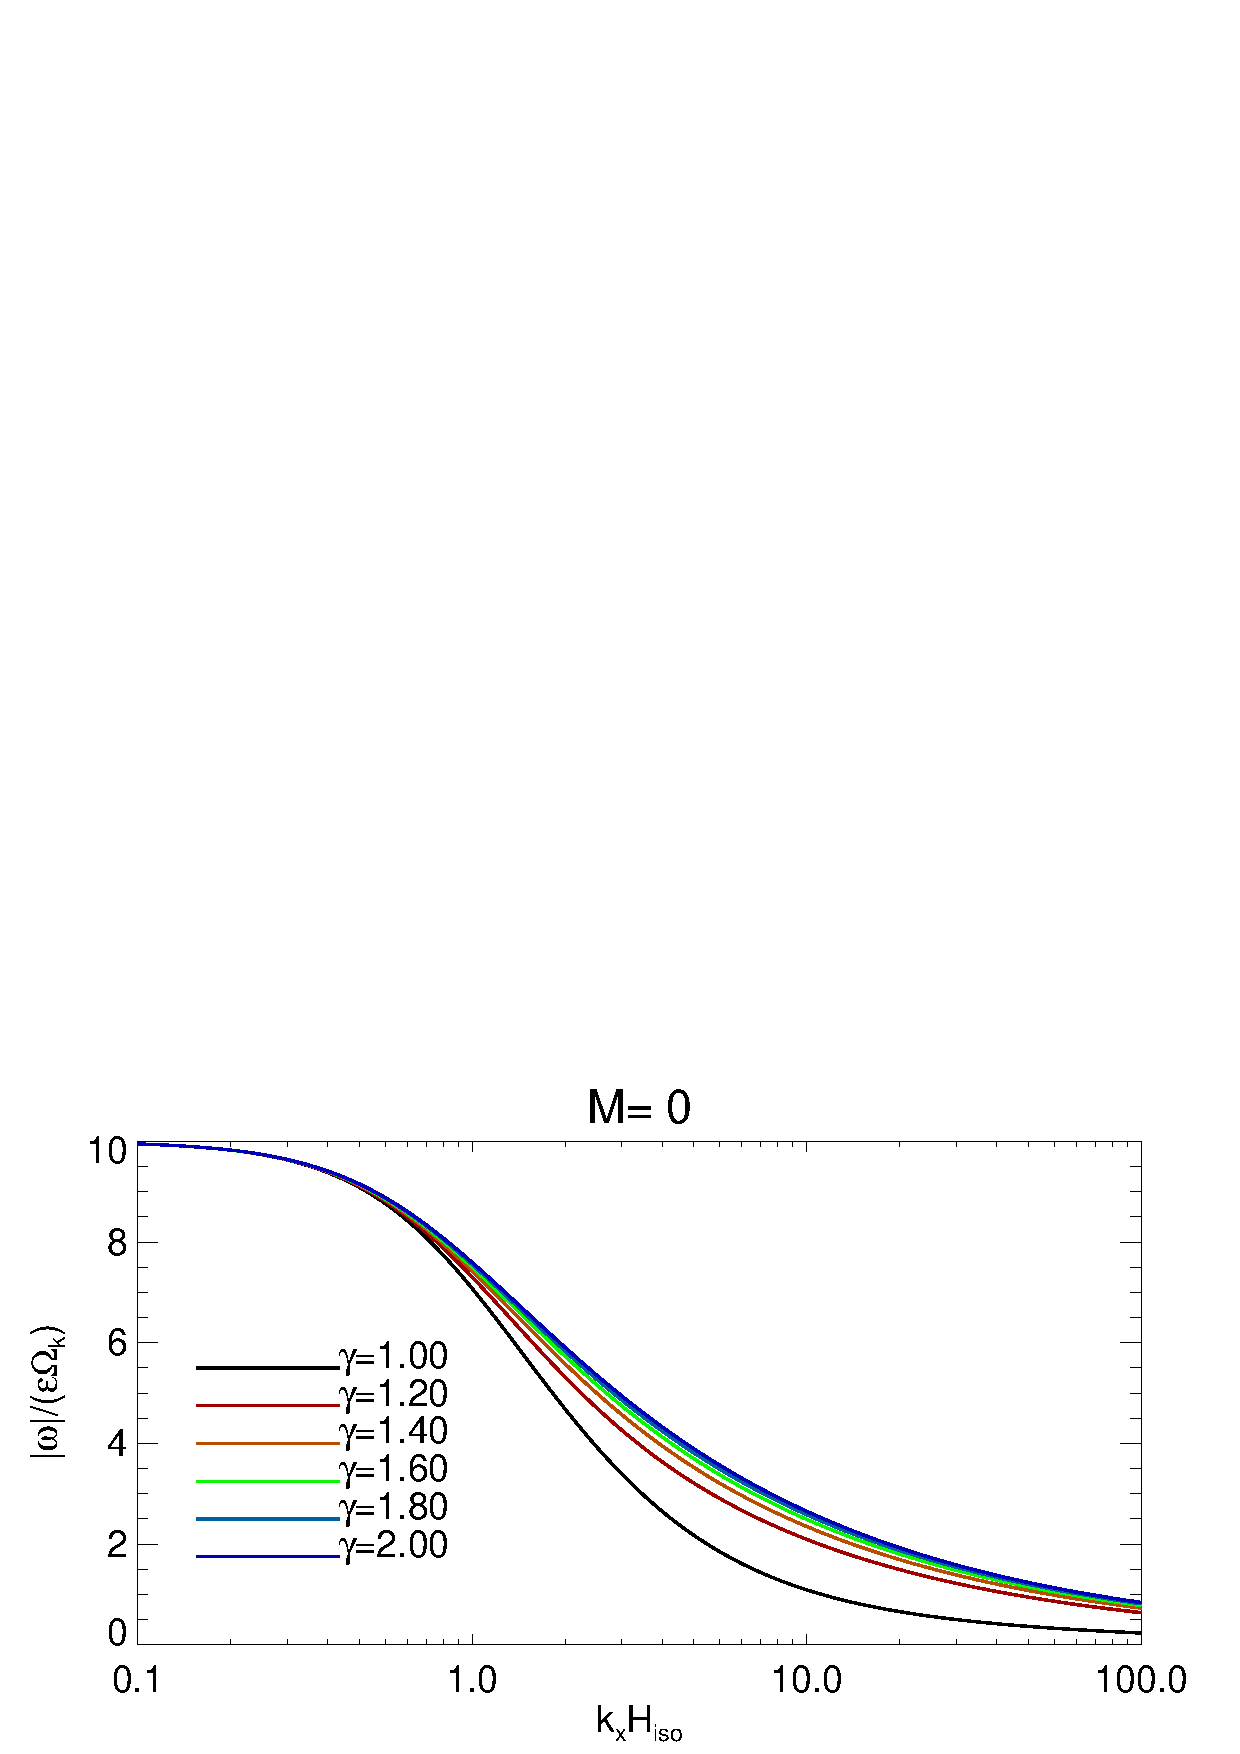
\includegraphics[width=\linewidth,clip=true,trim=0cm 1.75cm 0cm 0cm]{figures/rate_theory_om}
  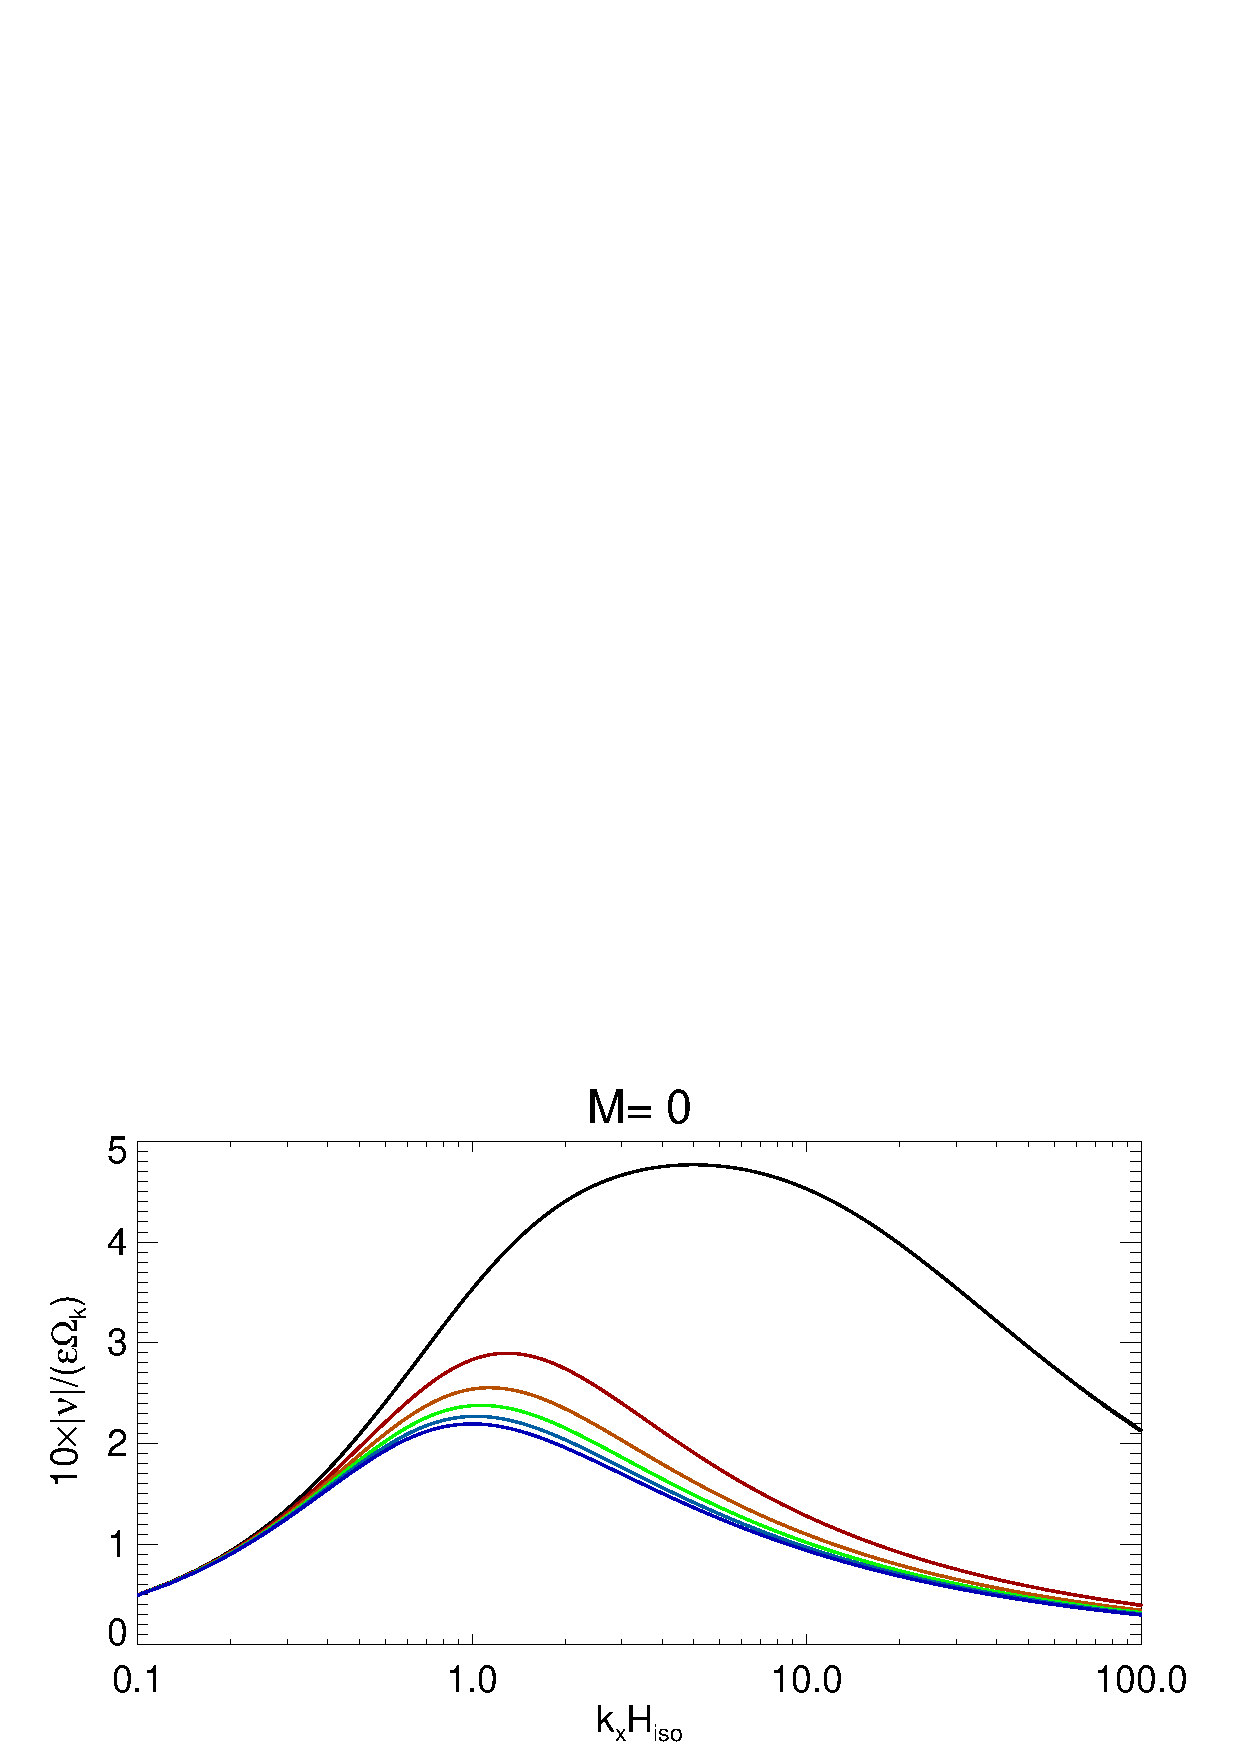
\includegraphics[width=\linewidth,clip=true,trim=0cm 0cm 0cm 1cm]{figures/rate_theory_nu}
  \caption{Real frequency (top) and growth rate (bottom) of the fundamental VSI mode in vertically 
    isothermal disks ($\Gamma=1$) subject to adiabatic perturbations,
    calculated in thin disk approximation from Eq. \ref{adia_disp}
    with $M=0$, $\epsilon=0.1$ and  
    $|q|=1$. Frequencies are shown as a function of the radial
    wavenumber for different values of the adiabatic index
    $\gamma$. For $\gamma\equiv 1$ the perturbations are isothermal
    and there is no vertical entropy gradient.\label{adia_growth}}  
\end{figure}   